\chapter{Background}\label{chap:background}

\section{The Skip-Gram Model} 
The Skip Gram Model is a model used to embed words into vectors, by analyzing the context in which the words happen. It's acheiving this by maximizing the following equation:\begin{equation} \label{basicSkip} \prod_{t=1}^T \prod_{-m<j<m}  p(w_{t+j}|w_t) \end{equation} Where T is the number of words in the corpus data, $w_i$ the $i-th$ word in the corpus data and $m$ is the context window. This means that the $m$ nearest words to $w$ are considered as context words.
This equation can be transformed quite easily into sums by using log probabilities: 
\begin{equation} \sum _{t=1}^T \sum_{-m<j<m} log( p(w_{t+j}|w_t) )\end{equation} 
    where the parameters are the same as in \ref{basicSkip}. The basic Skip-Gram Model uses a classical softmax to calculate the conditional probability $p(w_{t+j}|w_t)$: 
   \begin{equation}
   p(w_{t+j}|w_t)=  \frac{exp(w_{t+j}^T w_t)}{\sum_{w=1}^v exp(v_w^T w_t)}
   \end{equation}
  
  There lies a problem in this approach. As a matter of fact it is not feasible to compute the softmax. For the computation of $\sum_{w=1}^v exp(v_w^T w_t)$ one has to go over the whole corpus data. As very big data sets are needed to train the model, this is not a solution. But different solutions were proposed by \cite{mikolov2}. The first one is to use a Hierarchical soft max introduced by \cite{hsoftmax}. In this model the probability distribution of the output nodes is saved in a binary tree which gives one a logarithmic computation time for each of these probabilieties, and this makes it feasable to compute the softmax. Another possibility is the use of negative sampling which is used in the original word2vec implementation \cite{mikolov2}, which I shall discuss in the next section. 

\section{Negative Sampling}
The idea behind negative sampling is to only update the output nodes of certain words. This will obviously save an enormous amount of computation time. The idea is that given a pair $(x,c) \in D$, where $c$ is a word in the context window of $w$ we will set $p(x|c) =1$. Then select $K$ random words $k_i$ from the corpus data and set $p(x|k_i) = 0$, more one the random distribution later. We will denote the probability that the $(w,c)$ wasn't drawn at random the following way: $p(y=1|w,c)$, and if $(w,k) $ is chosen at random this way: $p(y=0|x,k)$.  Know we will use logistic regression to update the weights of the $k$ selected context words and $c$. By doing so we will only have to update $k+1$ output nodes.

Let's look at how we construct our objective function for a given word $w$ and one of its context words $c$: 

\begin{align*}
p(x|c) &= p(y=1|w,c) + \prod_{k\in K} p(y=0|k,c) 
\\&= p(y=1|w,c) + \prod_{k\in K} 1- p(y=1|k,c) 
\\&= log((p(y=1|w,c)) + \sum_{k\in K} log(1- p(y=1|k,c)) &&\text{Use of log probabilities}
\\&=  log(\frac{1}{1+e^{-v_c v_x }})  + \sum_{k\in K} log(1-\frac{1}{1+e^{-v_c v_k}}) &&\text{Use of softmax}	
\\&=  log(\frac{1}{1+e^{-v_c v_x }})  + \sum_{k\in K} log(\frac{1}{1+e^{v_c v_k }})
\\&= log(\sigma(v_c v_x ) + \sum_{k\in K} \sigma(log(-v_c v_k )) &&\text{$ where, \sigma = \frac{1}{1+e^{-x}}$}
\end{align*}

We see that to compute our objective function we will only have to compute the sum over $K$. Which in practice is very small (2-20). Too put things in perspective lets imagine our data set consists of 100000 words, we set $K=2$ and let's say that each output neuron has weight vector $v$ with $|v| = 300$. When updating our weights we would only update  $0.2*10^{-2}$ of the 300 million weights in the output layer. 

One question remains: how do we choose our random words? \cite{mikolov2} used the following random distribution:
 
 \begin{equation}
P(w)=\frac{f(w)^{\frac{3}{4}}}{\sum_{w_k\in W} f(w_k)^{\frac{3}{4}}}
\end{equation}
where $f(w)$ is the frequency of $w$ in the Vocabulary $W$. The value of $\frac{3}{4}$ is set empirically.

It's quite easily observable that this approach will outperform the classical softmax in computation time. Now the question arises if the accuracy is good enough enough but according to \cite{mikolov2} the negative sampling method "is an extremely simple training method that learns accurate representations". 
We know have enough background knowledge about word2vec and the skip gram model to look at how it can be optimized. In the next section we are going to cover what has already be done.

\section{Optimization of the Skip Gram Model}
Due to the popularity of the skip gram model, a lot of research went into optimizing it. This research can actually be divided into two categories, parallelization, and the optimization of the accuracy of the algorithm by allowing words to have multiple meanings. In this section we are going to cover.

\subsection{Parallelization}
In the original model the optimization is done with Stochastic Gradient Descent (SGD), which is a sequential algorithm. This does not favor a paralization process. To deal with this problem \cite{mikolov2} used a Hogwild tree proposed by \cite{hogwild}. The approach is to allow multiple threads to acces a shared memory, in this case the single model. This can obviously lead to overwriting errors. But according to \cite{hogwild} this doesn't lead to a significant accuracy loss if the data access isn't too frequent. But this maybe inaccurate for NLP, and especially for word embedding, as many words share the same context words. There were several attempts at solving this issue, and we are going to cover a few of them in the following subsections. 

\subsubsection{Parallization in shared and Distributed Memory}
The first parallization solution which was proposed by \cite{intel}, is to try to reduce the cost of our vector multiplication. The main idea in this paper is to convert the level 1-BLAS vector to vector operations to a level-3 BLAS matrix multiplication operation. This is achieved, buy using the same negative samples for each context word of a given word $w$. Instead of using for each context word a vector to vector multiplication we can transform this, under the assumption that we will not loose accuracy by sharing the same negative samples,  into a matrix multiplication. The matrix multiplication can be represented the following way.
\[
\begin{bmatrix}
w \\
w_{n_1}  \\
\vdots \\
w_{n_k}\\
\end{bmatrix}
*
\begin{bmatrix}
w_{c_1}\\
\vdots\\
w_{c_{2m}}\\
\end{bmatrix}
\]

where $w$ is our given word, $w_{n_1}...w_{n_k}$ are the shared negative samples, with $k \in [5,20]$, and $w_{c_1}...w_{c_2m}$ are the words inside of the context window $m$ of $w$, with $m \in [10,20]$, also called a batch of input context words. After each batch the model updates the weights of the used vectors. 
This model achieves a 3.6 fold increase in throughput, by only losing 1\% of accuracy. This model though is only applicable on architectures that are capable of such level-3 BLAS operations.
\subsubsection{Parallelization by the use of caching}
This idea was proposed by \cite{efficient}. The architecture used here is the basic skip gram model with an hierarchical soft max.  The general idea is to cache the most frequent used nodes of the binary tree used to memorize the probability distribution, and update them on the shared single model after a certain amounts of seen words (the paper used the number 10). The paper produced interesting results as they managed to increase efficiency by increasing the number of cores used for the calculation. This is very powerful because in the original implementation the accuracy regressed after 8 cores, this seems to indicate that too much overwriting is happening, as the number of concurrent threads surpasses a certain threshold. This can be seen in \ref{fig:efficient}, where c31 is the model proposed by \cite{efficient}
\begin{figure}[ht]
    \centering
			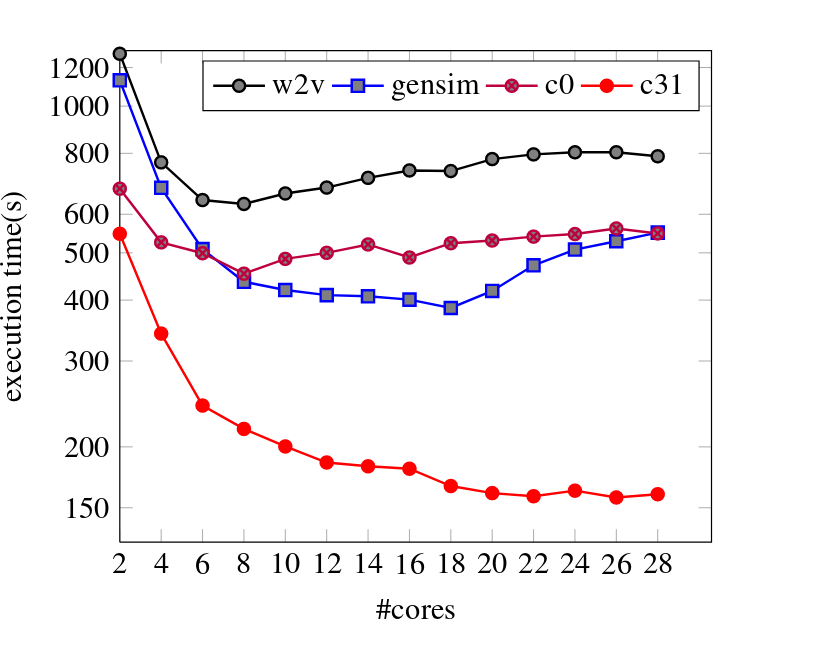
\includegraphics[scale=0.3]{images/cachingEfficiency.png} 
    \caption{Comparasion of the execution time in relation with the number of used cores \cite{efficient}}
    \label{fig:efficient}
\end{figure}
%%%%%%%%%%%
\iffalse
\subsection{Restating the problem as Matrix factorization}
It was also shown in \cite{goldenberger} that the optimization problem solved by the sgd can alos be restated as a matrix factorization. In fact the partial derivative Matrix W*C where w is the word embedding matrix and C the context matrix, is nothing else then PPMI - log k. which states the optimizing problem as a pure matrix factorization problem. Also this first step showed similar results to the original word2vec. Then this was picked up by, to do it with riemman  optimization and outperformed the original word2vec in accuracy. 
\fi
%%%%%%%%%%%

\subsection{Context sensitive word embedding}
A word does not always have the same meaning according to it's context. This is a problem that is not addressed by word2vec and the general skipGram model. Some new models, that have taken this issue into consideration, were proposed. A lot of work has be done in this direction, \cite{topicalWE},  \cite{breaking} for example, but the the one reporting the best results is \cite{contextWithTensor}. The main idea is to change the way we compute the and variables we use in our conditional probability. The idea is to look if a word given a certain context word matches to a topic. Bank would match too finance given the context word money. Bank would also match too nature if river was the given context word. But bank would not match too nature with the context word money. Now this arises the questions of how one could achieve this, first we have to introduce new variables, for this let's look at the objective function used: 
First let's take a look at the objective function:
\begin{equation}
J(\Omega) = \sum_{(w,t,c)\in D} \sum_{(w,\tilde{t},\tilde{c} \in{\tilde{D}})} max(0,1- g(w,t,c) + g(w,\tilde{t},\tilde{c})) \lambda||\Omega||_{2}^2
\end{equation}

This approach uses the same negative sample technique as described in the previous sections, $D$ is the corpus data and $\tilde{D}$ is the set of negative samples and $\lambda$is the hyperparameter used for the standard $L_2$ standarization. What is interesting here is the function $g(w,c,t)$, where $w$ is a word, $c$ the context word, and $t$ the context in which the word appears, $g$ is defined as follows: 
\begin{equation}
g(w,c,t) = u^T \sigma(w^TM^{[1:k]}t+V_c^T(w \oplus t) + b_c)
\end{equation}
where, $u, V_c, b_c$ are standard parameters for a neural network, $\oplus$ is the vector concatenation, while the most important parameter is $M^{[1:k]}$, which a tensor layer, the tensor layer is used because of its ability to model multiple interactions in the data, as this will be useful for multiple contexts. They used SGD for the optimization of this objective function.  They achieved really interesting results as shown in \ref{fig:multipleContext}.
\begin{figure}[ht]
    \centering
			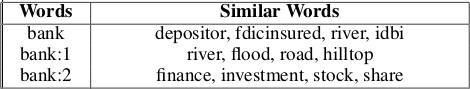
\includegraphics[scale=0.7]{images/multipleContext.png} 
    \caption{"Nearest  neighbor  words  by  our  model  and  Skip-
Gram. The first line in each block is the results of Skip-Gram;
and the rest lines are the results of our model" \cite{contextWithTensor}}
    \label{fig:multipleContext}
\end{figure}



